\subsection{Online TD3BC with Jump-Starting Privileged Actor}\label{sub:seq_snn}
To address the aforementioned challenges in sequential SNN training, we adapt the Jump-Start Reinforcement Learning (JSRL) framework \cite{Uchendu2022}. It leverages a pre-trained guide policy to create a curriculum of starting conditions for a secondary policy. We implement a privileged, non-spiking actor, trained for a few epochs through TD3 \cite{fujimoto2018addressing}, training is stopped when the policy can hover the drone for the warm-up period consistently. Its primary function is to bridge the critical warm-up period required by the SNN. Both the guiding policy and the non-spiking critic receive privileged information in the form of action histories. 

A replay buffer is continuously populated throughout training with transitions generated by both the guiding actor (during the initial warm-up phase) and the spiking policy (during subsequent interactions). This hybrid approach bridges the early training period, where the spiking policy still gathers short sequences. Therefore, supervised learning from the guiding policy interactions is effective during early training. 

The guide controller, which receives a privileged set of observations, including the action history, is used for the first $500-N$ timesteps, after which the spiking policy interacts for the remaining $N$ steps, linearly increasing $N$ until the guide policy is only used for the warm-up period. Initially, the buffer is filled mostly with experience from the guiding policy. This introduces a risk of training a spiking policy that closely resembles the guide policy, which can be undesirable as the guide is usually not an expert policy. Therefore, the choice of the BC term weight is crucial to prevent the spiking policy from overfitting to the guide policy.

Once our spiking policy gains a baseline performance, and generates sufficiently long rollouts, we want to leverage the reward information, for which online RL is better suited. Inspired by TD3BC \cite{FujimotoMinimal}, we incorporate a Behavioral Cloning (BC) term into the RL objective function that utilizes the guide policy demonstrations stored in the replay buffer. The BC weight \(\lambda\) decays exponentially, shifting from imitation to reward-based optimization. The BC term in our approach serves two purposes: avoiding large changes in policy behavior, improving training stability, and leveraging the demonstration data efficiently. 

We call this approach TD3BC+JSRL, pseudocode can be found in \autoref{sup:pseudo}. The objective to be maximized can be defined as:

\begin{align}
    J_{\pi}
    &= \mathbb{E}_{\mathbf{\tau} \sim \mathcal{D}}
    \left[
        \sum_{i=0}^{n_{\text{seq}}-1}
        \mathbf{1}_{\mathrm{i\geq n_{warm-up}}}
        \Big(
            Q_{\phi_1}\big(
                \mathbf{s}_{\tau,i},
                \pi_{\theta}(\mathbf{s}_{\tau,i} \mid \mathbf{h}_{\tau,i})
            \big)
            - \lambda
            \big\|
                \pi_{\theta}(\mathbf{s}_{\tau,i} \mid \mathbf{h}_{\tau,i})
                - \mathbf{a}_{\tau,i}
            \big\|^2
        \Big)
    \right].
\end{align}


Where the history, $\mathbf{h_{\tau, i}}$, is defined as:
\begin{align}
    \mathbf{h}_{\tau,i} &:= (\mathbf{s}_{\tau,0}, \mathbf{s}_{\tau,1}, \dots, \mathbf{s}_{\tau,i-1}), \\
    \mathbf{h}_{\tau,0} &:= \varnothing.
\end{align}


% function needs to be checked
\( Q_{\phi_1} \) in the first term represents the first critic network, as used in TD3. The variable \( \tau \) denotes a sequence sampled from the replay buffer, with a length of $n_{seq}=100$. Within this sequence, \( \mathbf{s}_{\tau,i} \) and \( \mathbf{a}_{\tau,i} \) correspond to the \( i^\text{th} \) observation and action, sampled from the replay buffer, respectively. The hyperparameter \( \lambda \) controls the strength of the BC regularization and decays exponentially over time; the BC coefficient $\lambda$ starts at $\lambda_0 = 0.2$ and decays exponentially ($\lambda \leftarrow 0.99\lambda$) after each epoch, shifting emphasis from imitation to reward optimization as training stabilizes.
When the guiding policy is of high quality, a larger \( \lambda \) is preferred. Finally, \( \mathbf{1}_\mathrm{i\geq n_{warm-up}} \) equals zero during the warm-up period ($\mathrm{n_{warm-up}}$), which in our case is $50$ steps, corresponding to $0.5$ seconds in the drone control task. We zero-initialize hidden states, which causes only marginal performance differences \cite{Kapturowski2019}. The critic is not time variant and thus does not need a warm-up period.

\subsection{Spiking Neural Networks for Continuous Control}\label{subsection:S-AC}
Spiking Neural Networks leverage bio-inspired neuron models, which transmit information through binary spikes. The membrane potential is charged by an input current \( I_{in} \), which incrementally charges its membrane potential \( U \). Over time, the potential decays at a rate determined by the leak factor \( \beta \). When the membrane potential exceeds a defined threshold \( U_{thr} \), the neuron emits a spike, \( s\), and its potential is subsequently reset. We employ a soft-reset spiking mechanism, which is described by:

\begin{equation}
U[t+1] = \beta U[t] + I_{in}[t+1] - s \cdot U_{thr}, \quad \text{where } s = \begin{cases}
1, & \text{if } U[t] > U_{thr} \\
0, & \text{otherwise}
\end{cases}
\end{equation}

Hence, the spiking function $f(U[t])$ is the non-differentiable Heaviside function and calls for surrogate gradients \cite{NeftciSurrogate} to enable gradient based optimization methods. During the backward pass, we act as if this Heaviside function was a parametrized sigmoid function, $\sigma(kx)$, which is the true when $k \rightarrow \infty$. For computational efficiency, the gradient of this parametrized sigmoid is approximated by the gradient of fast sigmoid (\(fs(k\cdot x) = \frac{k\cdot x}{1+k\cdot |x|}\) ) \cite{zenke2018superspike}. To avoid exploding gradients, the actual gradient of the fast sigmoid is normalized by $k$, which leaves us with the derivative in \autoref{eq:grad_fast_gradient}; 
\begin{equation}\label{eq:grad_fast_gradient}
\frac{d }{dx}fs(k\cdot x)\cdot \frac{1}{k} = \frac{k}{(1+k\cdot |x|)^2}\cdot \frac{1}{k} = \frac{1}{(1+k\cdot |x|)^2}, 
\end{equation}
where a larger $k$ relates to a steeper slope of the parametrized sigmoid, reducing the range of inputs for which a gradient exists. 

SNNs work in a spike-based domain. To encode continuous values to spikes and vice versa, population based encoding and decoding are used. Specifically, the first linear layer encodes continuous input values into currents, and a final layer decodes the output spikes into motor commands. This approach has been proven successful in previous work \cite{stroobants2025neuromorphic}. 

Our  controller is a feedforward SNN with input size $18$, two hidden layers and $4$ output neurons. The two hidden layers of the network are of size $256$ and $128$ respectively and make use of Leaky Integrate-and-Fire neurons. This architecture enables analysis of surrogate gradient effects across multiple layers, sufficient capacity for continuous control, and is small enough for deployment on the resource constrained Crazyflie.


\subsection{Surrogate Gradients in Deep Networks}\label{sub:surrgradsched}
\begin{figure*}[ht!]
    \centering
    \begin{subfigure}[t]{0.31\textwidth}
        \centering
        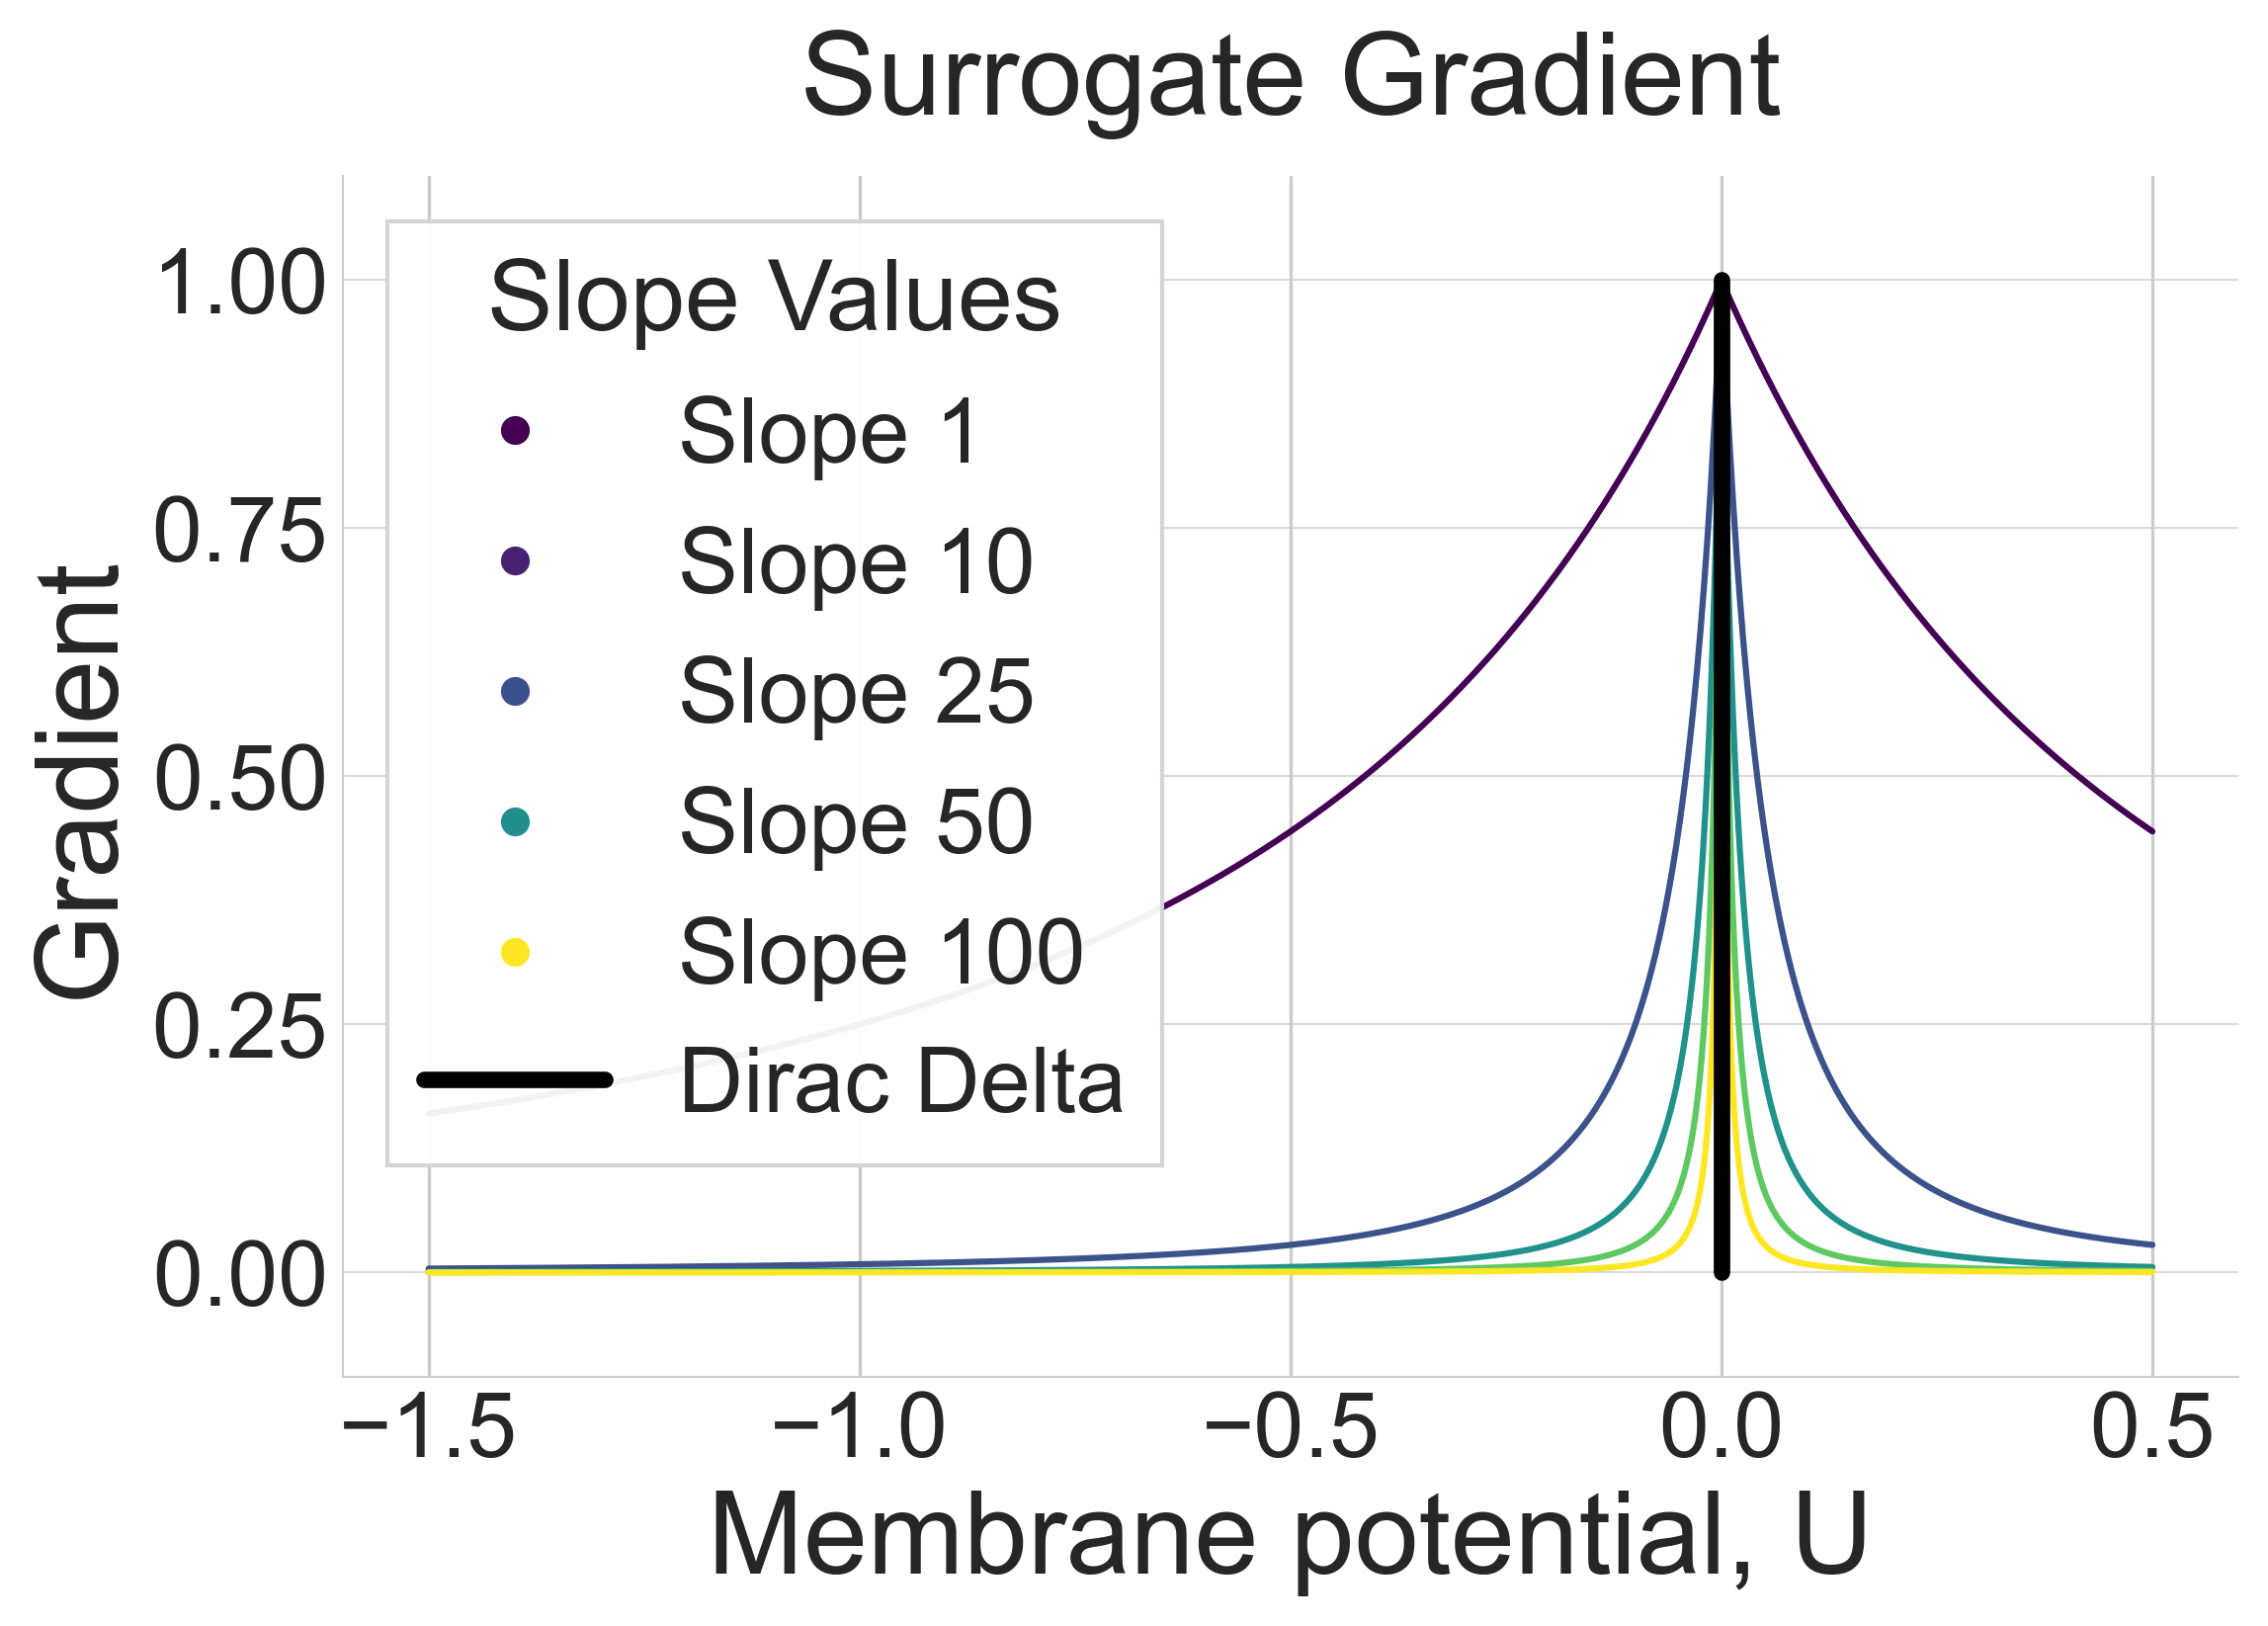
\includegraphics[height=3.6cm]{figures/neurips_surrogate_gradients.png}
        \caption{The slope of the surrogate gradient dictates the range of inputs for which a gradient exists.}
        \label{fig:surrslope}
    \end{subfigure}
    \hspace{0.02\textwidth}
    \begin{subfigure}[t]{0.31\textwidth}
        \centering
        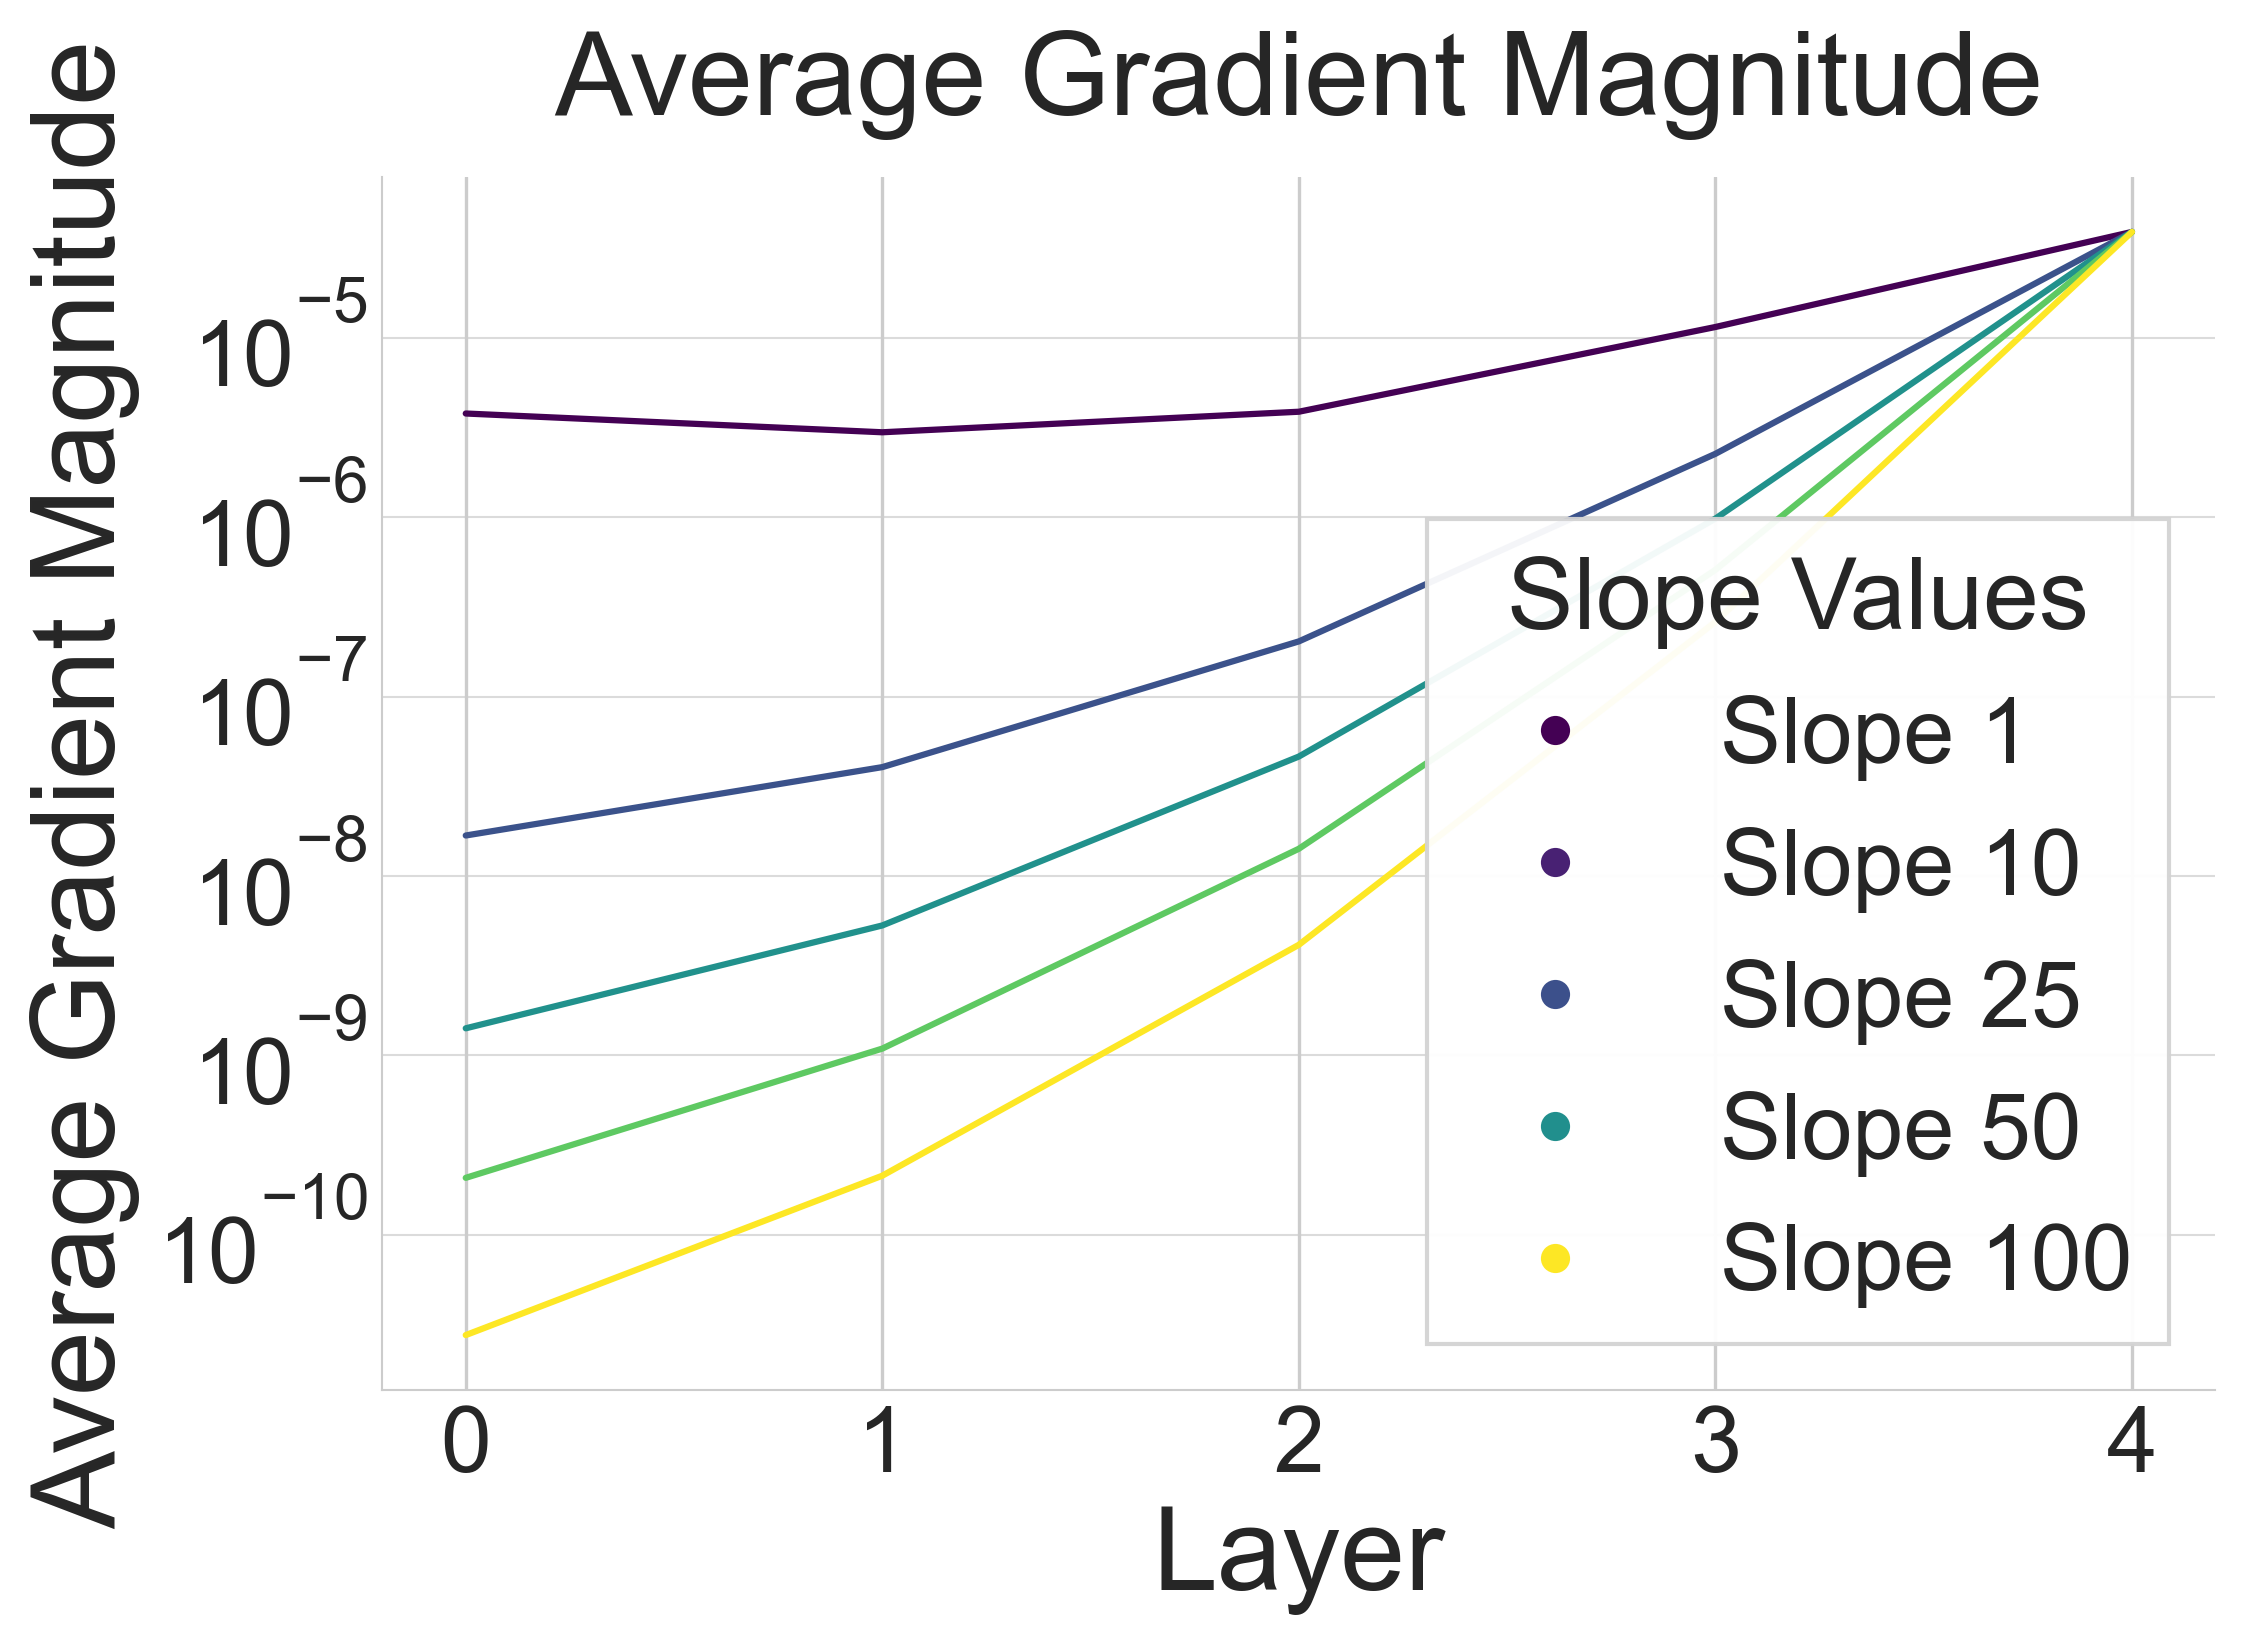
\includegraphics[height=3.6cm]{figures/neurips_avg_grad_magnitude.png}
        \caption{A more shallow slope carries the gradient deeper through the network, suffering less from vanishing gradients.}
        \label{fig:gradmagn}
    \end{subfigure}
    \hspace{0.02\textwidth}
    \begin{subfigure}[t]{0.31\textwidth}
        \centering
        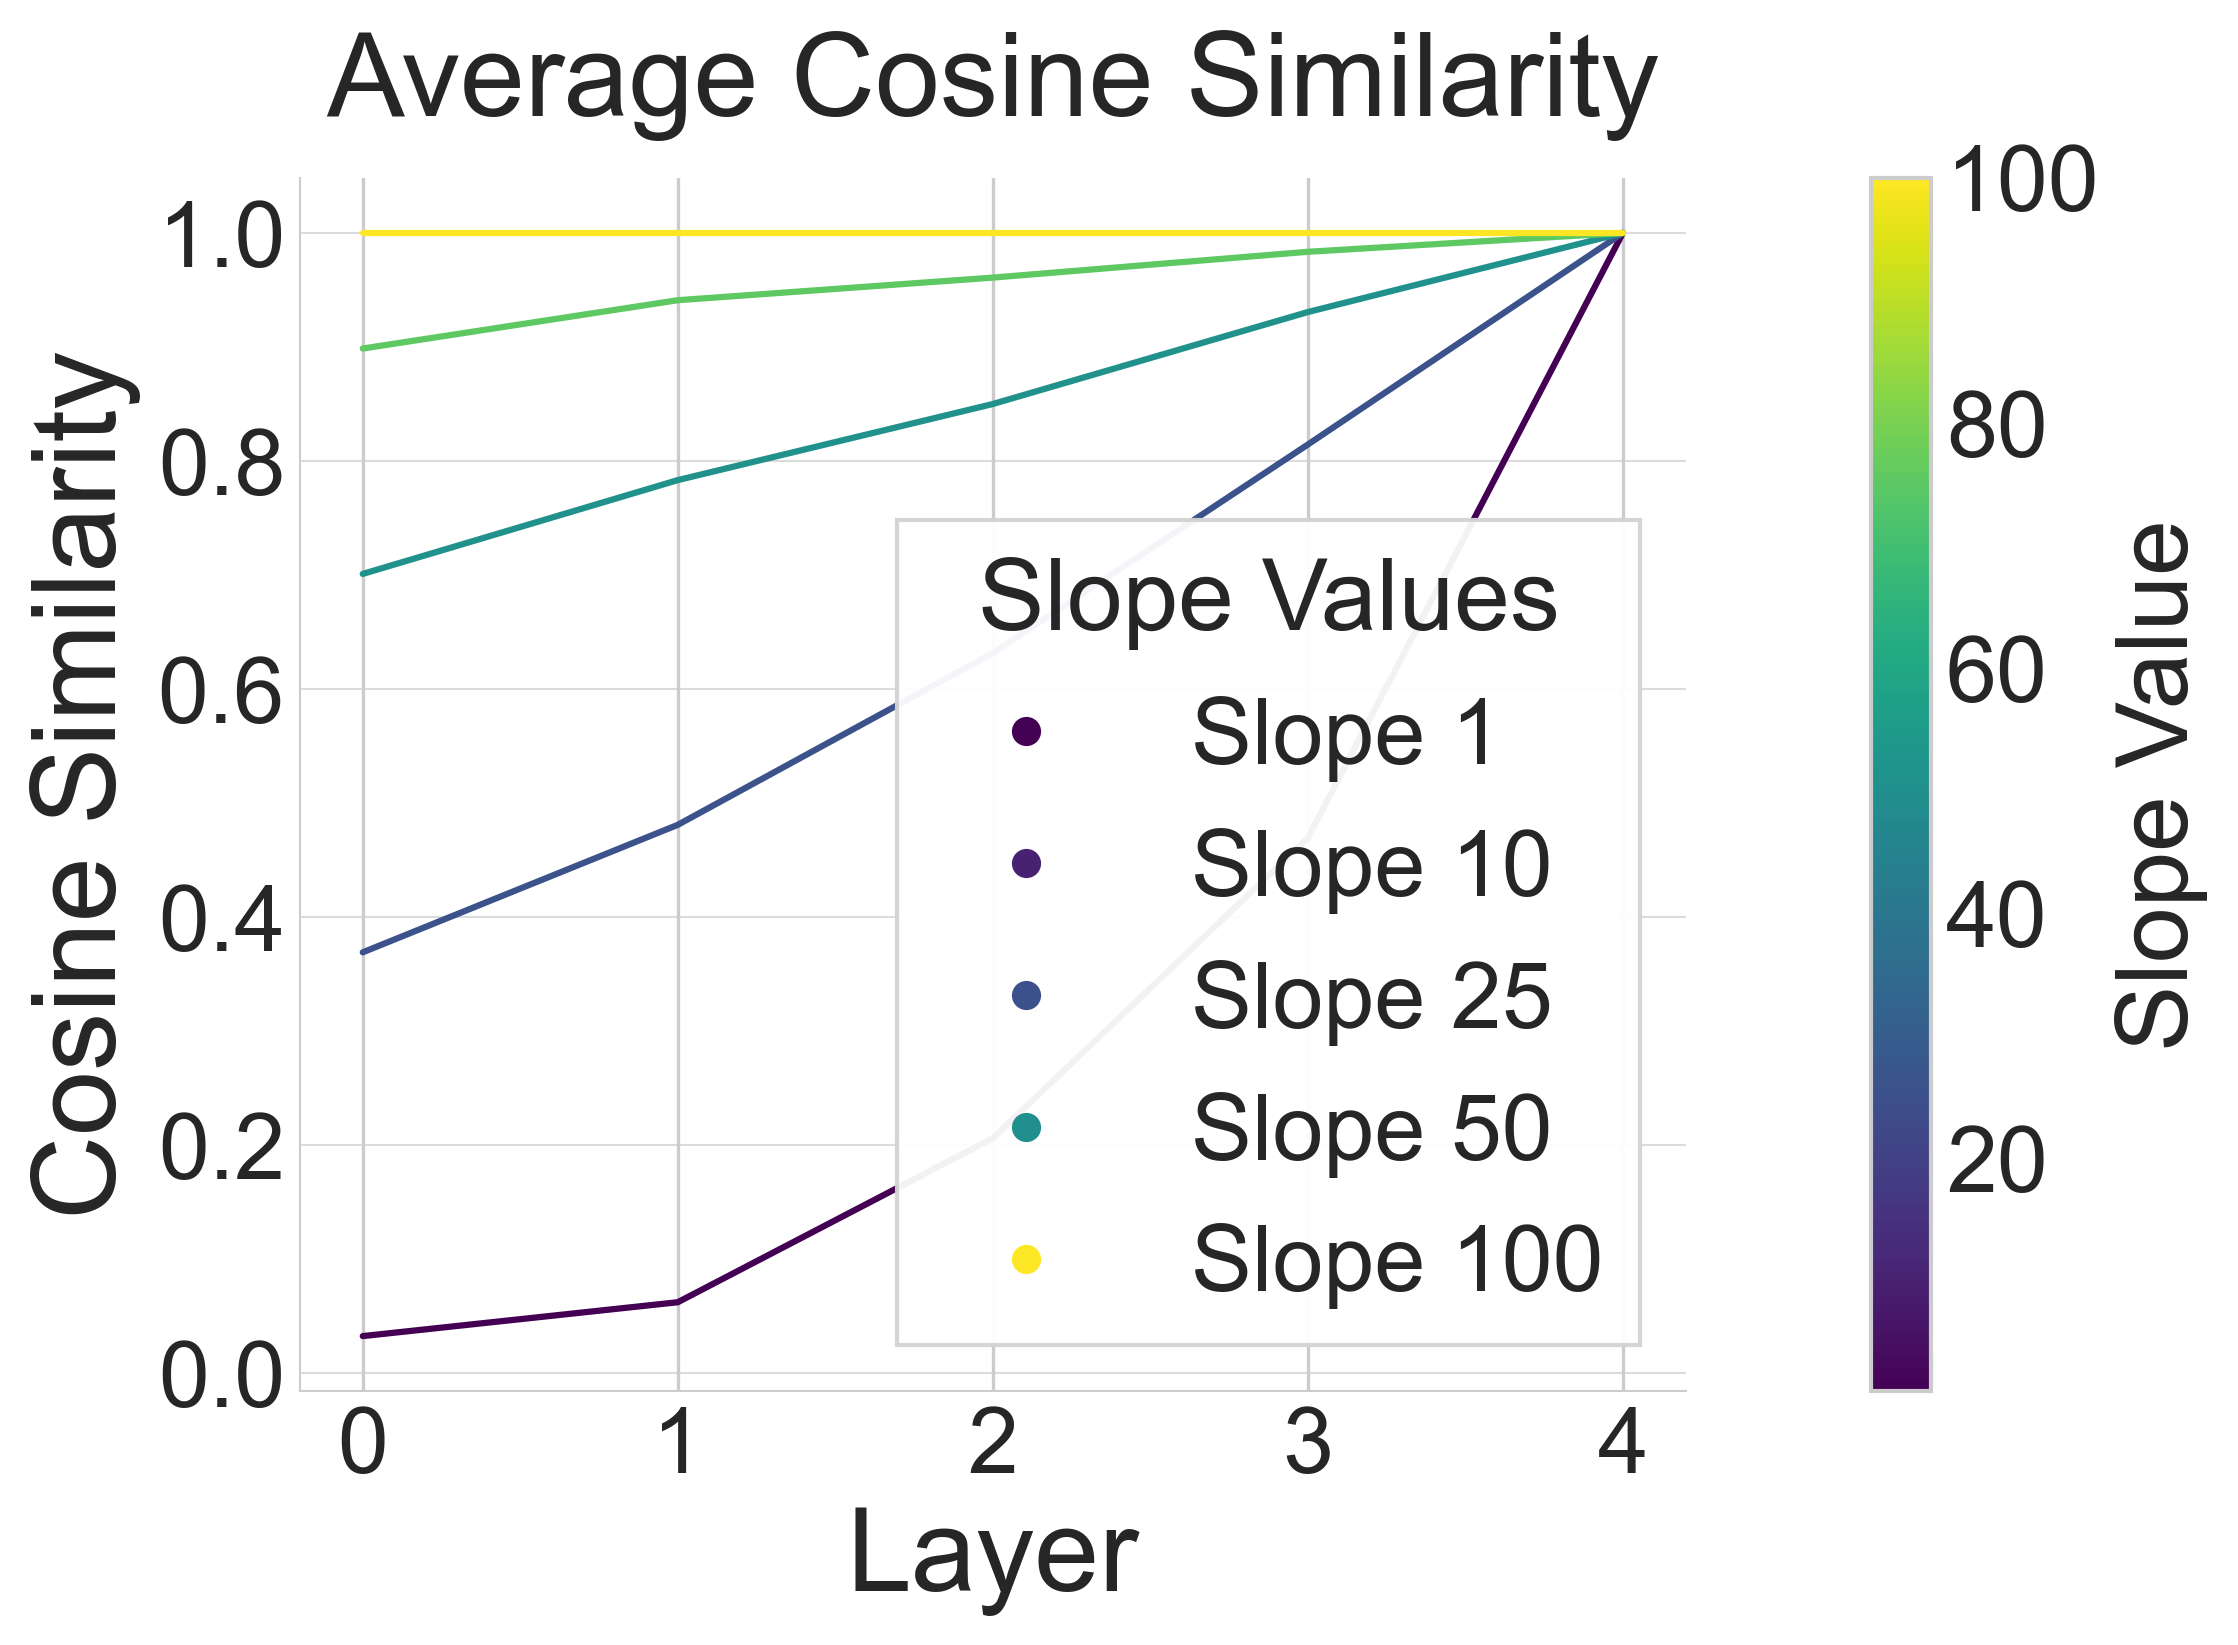
\includegraphics[height=3.6cm]{figures/neurips_cosine_similarity_line.png}
        \caption{A shallower slope introduces bias and variance, computed using the cosine similarity. }
        \label{fig:cossim}
    \end{subfigure}
    
    \caption{Surrogate gradient slope-magnitude-alignment tradeoff in deep SNNs. (\ref{fig:surrslope}) Shallow slopes ($k{=}1$) provide gradients over wider input range than  steep slopes ($k{=}100$). (\ref{fig:gradmagn}) This prevents vanishing gradients in deeper layers, critical for multi-layer SNN training. (\ref{fig:cossim}) However, shallow slopes introduce directional noise (cosine similarity $\to$ 0), which aids RL exploration but hinders supervised convergence. Network: 4 layers of 64 neurons; layer 0 = first hidden, layer 4 = output.}
    \label{fig:fullwidthfigure}
\end{figure*}
Training SNNs via backpropagation requires the use of surrogate gradients to approximate the derivative of the non-differentiable spike function. A critical hyperparameter in this process is the slope $k$ of the surrogate function, which determines the sensitivity of the gradient near the spiking threshold.

We adopt the gradient of a fast sigmoid function, see \autoref{eq:grad_fast_gradient}, and examine slope configurations ranging from shallow ($k = 1$) to steep ($k = 100$). We analyze a $4$ layer SNN, with all layers having $64$ neurons, layer $0$ corresponds to the input layer, while layer $4$ relates to the output. The results on the plots are the average of running the test $100$ times. As shown in \autoref{fig:surrslope}, steeper slopes closely resemble the Dirac delta function but restrict non-zero gradients to a narrow input range. In contrast, shallower slopes lead to a broader range of non-zero gradients. This increases the average gradient magnitude, particularly in deeper layers (\autoref{fig:gradmagn}). Note that the average gradient magnitude is influenced by the proportion of neurons with zero gradients in each layer. 
% Individual neurons that do receive a gradient will have values within the range $[0, 1]$, as shown in \autoref{fig:surrslope}. The very low average values (e.g., around $10^{-10}$ for $k = 100$) thus reflect sparsity in gradient propagation rather than gradients falling below machine precision.

While the surrogate gradient's slope affects the quantity of weight updates per backward pass, it also introduces noise into the gradient computation~\cite{GygaxElucidating}. Since the true gradient for deeper network layers does not exist, we analyze the relationship between a steep surrogate gradient ($k=100$), which approximates the true gradient $\nabla W_i$ more truthfully than a shallow slope, and shallow surrogate gradients, denoted as $\tilde{\nabla}W_i$, using cosine similarity:
\begin{equation}
\text{cosine similarity} = \frac{\mathbf{\nabla W}_i \cdot \mathbf{\tilde{\nabla}W_i}}{\|\mathbf{\nabla W}_i\| \|\mathbf{\tilde{\nabla}W_i}\|}.
\end{equation}
\autoref{fig:cossim} shows that the cosine similarity for shallow slopes reduce to $0$, therefore, the weight updates in deeper networks become essentially random.

We propose an adaptive surrogate gradient scheduling approach. Shallow slopes, which introduce stochasticity into the gradient computation, can facilitate the update of a broader set of connections in deeper networks, enhancing exploration in RL, and increase the gradient magnitude. Conversely, steep slopes yield more precise gradient estimates, which are advantageous once the agent’s performance stabilizes and fine-tuned optimization is desired. This mechanism provides a natural means of balancing exploration and exploitation throughout training.

Three schedules are analyzed:
\begin{itemize}
    \item \textit{Fixed}: The surrogate gradient slope is held fixed throughout training.
    \item \textit{Interval}: The surrogate gradient slope is made steeper according to a fixed time schedule.
    \item \textit{Adaptive}: The surrogate gradient slope is adapted as function of the achieved reward.
\end{itemize}
% Adaptive scheduling uses a weighted sum of the low-passed first order derivative of the reward score history and the low-passed reward score itself, see \autoref{eq:adaptive}. 
The adaptive slope scheduler tracks both the reward value and its derivative (see \autoref{eq:adaptive}), allowing the slope to increase when performance improves and stabilize once it saturates. This keeps the gradient noisy when exploration is needed and sharp when fine-tuning.
Note that the term depending on $r_{t-i}$ is largely responsible for maintaining the slope when maximum performance is reached, and thus prevents destroying progress.
\begin{equation}\label{eq:adaptive}
    k_t = \frac{1}{10} \sum_{i=0}^{9} \left[0.5 r_{t-i} + 0.5 r'_{t-i}\right],
\end{equation}
where $k_t$ is the slope at time $t$, $r_{t-i}$ is the reward score at time $t-i$ and $r'_{t-i}$ is the first order derivative of the reward score at time $t-i$.
Furthermore, $k$ is clamped between 1 and 100, the same limits as used in~\autoref{fig:fullwidthfigure}. 

% \KVDB{Its not really the equation I implement cause I first calculate U t+1 and then do the reset, but in one line it takes less space, is this fine?}


% Note that this is a first order model, which means that a large input essentially immediately causes a spike to be generated. In situations where an incoming spike should affect a neuron at a later time step, second order models could be more effective. 
% \KVDB{I DON'T KNOW IF THIS SHOULD OR SHOULD NOT BE MENTIONED, AT CONFERENCES, MANY 'OLD SCHOOL' NEUROMORPHS GOT A BIT ANNOYED BY FIRST ORDER MODELS RECEIVING SO MUCH PRAISE, AND WHEN USING EG IMU, WHERE INTEGRATION ETC IS NEEDED, SECOND ORDER MODELS ARE PROBABLY MORE EFFECTIVE? (NEXT TO FIXING SOME CONSTANTS TO 1 ;), CAN ALSO INCLUDE A FIGURE OR APPENDIX ON THIS, I HAVE SOME FIGURES ANYWAYS}

\subsection{Asymmetric Actor-Critic}
While the actor is spiking,  the critic is a feedforward ANN, which receives all observed states and an action history of 32 timesteps. This asymmetric setup has been demonstrated to successfully leverage the improved training stability of ANN \cite{Tang2020, Tang2020_Hardware}. The jump-starting actor used in this work, is also an ANN network with the same privileged inputs as the critic. 
% Please note that the critic is only used during training and is not deployed on the drone at inference time.
This critic is only used to stabilize training, and is not deployed on the drone at inference time.

